% Options for packages loaded elsewhere
\PassOptionsToPackage{unicode}{hyperref}
\PassOptionsToPackage{hyphens}{url}
%
\documentclass[
]{article}
\usepackage{amsmath,amssymb}
\usepackage{lmodern}
\usepackage{iftex}
\ifPDFTeX
  \usepackage[T1]{fontenc}
  \usepackage[utf8]{inputenc}
  \usepackage{textcomp} % provide euro and other symbols
\else % if luatex or xetex
  \usepackage{unicode-math}
  \defaultfontfeatures{Scale=MatchLowercase}
  \defaultfontfeatures[\rmfamily]{Ligatures=TeX,Scale=1}
\fi
% Use upquote if available, for straight quotes in verbatim environments
\IfFileExists{upquote.sty}{\usepackage{upquote}}{}
\IfFileExists{microtype.sty}{% use microtype if available
  \usepackage[]{microtype}
  \UseMicrotypeSet[protrusion]{basicmath} % disable protrusion for tt fonts
}{}
\makeatletter
\@ifundefined{KOMAClassName}{% if non-KOMA class
  \IfFileExists{parskip.sty}{%
    \usepackage{parskip}
  }{% else
    \setlength{\parindent}{0pt}
    \setlength{\parskip}{6pt plus 2pt minus 1pt}}
}{% if KOMA class
  \KOMAoptions{parskip=half}}
\makeatother
\usepackage{xcolor}
\IfFileExists{xurl.sty}{\usepackage{xurl}}{} % add URL line breaks if available
\IfFileExists{bookmark.sty}{\usepackage{bookmark}}{\usepackage{hyperref}}
\hypersetup{
  hidelinks,
  pdfcreator={LaTeX via pandoc}}
\urlstyle{same} % disable monospaced font for URLs
\usepackage[margin=1in]{geometry}
\usepackage{longtable,booktabs,array}
\usepackage{calc} % for calculating minipage widths
% Correct order of tables after \paragraph or \subparagraph
\usepackage{etoolbox}
\makeatletter
\patchcmd\longtable{\par}{\if@noskipsec\mbox{}\fi\par}{}{}
\makeatother
% Allow footnotes in longtable head/foot
\IfFileExists{footnotehyper.sty}{\usepackage{footnotehyper}}{\usepackage{footnote}}
\makesavenoteenv{longtable}
\usepackage{graphicx}
\makeatletter
\def\maxwidth{\ifdim\Gin@nat@width>\linewidth\linewidth\else\Gin@nat@width\fi}
\def\maxheight{\ifdim\Gin@nat@height>\textheight\textheight\else\Gin@nat@height\fi}
\makeatother
% Scale images if necessary, so that they will not overflow the page
% margins by default, and it is still possible to overwrite the defaults
% using explicit options in \includegraphics[width, height, ...]{}
\setkeys{Gin}{width=\maxwidth,height=\maxheight,keepaspectratio}
% Set default figure placement to htbp
\makeatletter
\def\fps@figure{htbp}
\makeatother
\setlength{\emergencystretch}{3em} % prevent overfull lines
\providecommand{\tightlist}{%
  \setlength{\itemsep}{0pt}\setlength{\parskip}{0pt}}
\setcounter{secnumdepth}{-\maxdimen} % remove section numbering
\ifLuaTeX
  \usepackage{selnolig}  % disable illegal ligatures
\fi

\author{}
\date{\vspace{-2.5em}}

\begin{document}

\hypertarget{epidemiological-studies-meta-analysis}{%
\section{Epidemiological Studies: Meta
Analysis}\label{epidemiological-studies-meta-analysis}}

The goal of epi.meta.analysis is to:

\begin{itemize}
\tightlist
\item
  Exhaustively Explore epidemiological research studies to figure out
  the regional (country wise) PM2.5 exposure range covered in these
  studies.
\item
  Identify and plot the locations of these studies on a map to identify
  locations where no/very few cohort studies have been undertaken.
\item
  Better understand the relationship between PM2.5 and Mortality/Life
  Expectancy.
\end{itemize}

\newpage

\hypertarget{analysis-and-plots}{%
\section{Analysis and Plots}\label{analysis-and-plots}}

\begin{itemize}
\tightlist
\item
  Note: All data that is used to generate the graphs below can be found
  in the \texttt{data-raw} sub-directory, which is present at the root
  of the \texttt{epi.meta.analysis} directory.
\end{itemize}

\hypertarget{pm2.5-distributions-of-the-lower-limits-and-upper-limits-of-exposure-range-density-and-histogram-plots}{%
\subsection{PM2.5 distributions of the lower limits and upper limits of
exposure range (Density and Histogram
Plots)}\label{pm2.5-distributions-of-the-lower-limits-and-upper-limits-of-exposure-range-density-and-histogram-plots}}

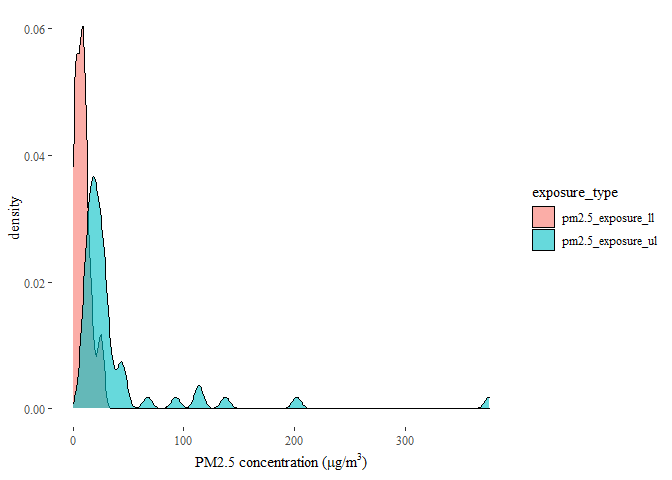
\includegraphics[width=1\linewidth]{man/figures/README-pm2.5_expo_ul_ll-1}
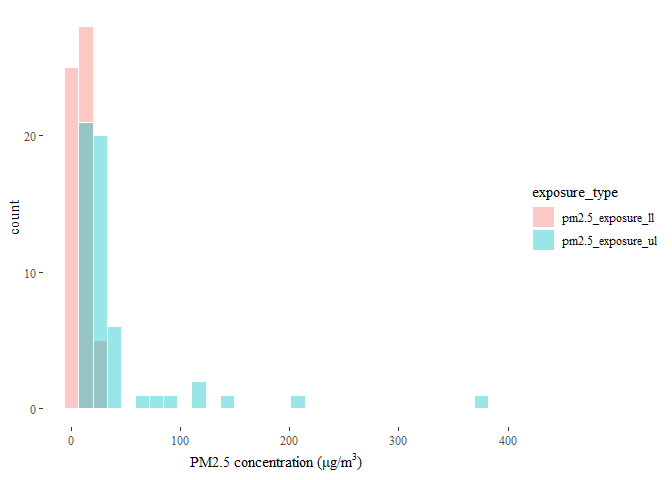
\includegraphics[width=1\linewidth]{man/figures/README-pm2.5_expo_ul_ll-2}

\begin{itemize}
\tightlist
\item
  From \textbf{Plot 1}, it looks like most of the studies are present in
  concentration ranges that are less than 50 µg/m³. According to AQLIs
  latest estimates, 12.6 percent (\textasciitilde962 million people) of
  the world population live in areas where PM2.5 pollution concentration
  is greater than 50 µg/m³.
\end{itemize}

\hypertarget{country-wise-mean-pm2.5-distribution-density-plot-and-historgram}{%
\subsection{Country Wise Mean PM2.5 distribution (Density Plot and
Historgram)}\label{country-wise-mean-pm2.5-distribution-density-plot-and-historgram}}

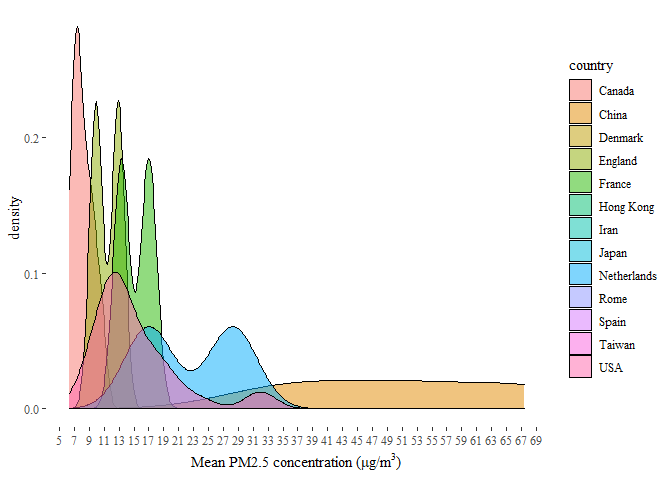
\includegraphics[width=1\linewidth]{man/figures/README-mean_pm2.5_country_wise-1}
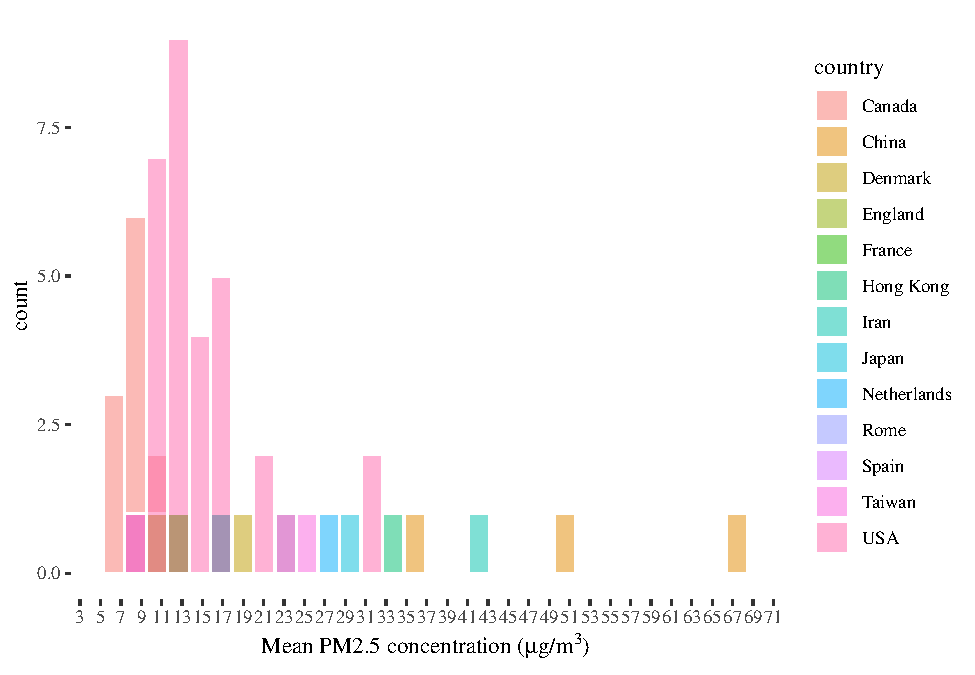
\includegraphics[width=1\linewidth]{man/figures/README-mean_pm2.5_country_wise-2}

\hypertarget{choropleth-world-map-mapping-the-total-number-of-epidemiological-studies-specifically-those-that-are-trying-to-better-understand-the-relationship-between-pm2.5-and-mortalitylife-expectancy.}{%
\subsection{Choropleth world map: mapping the total number of
epidemiological studies (specifically those that are trying to better
understand the relationship between PM2.5 and Mortality/Life
Expectancy).}\label{choropleth-world-map-mapping-the-total-number-of-epidemiological-studies-specifically-those-that-are-trying-to-better-understand-the-relationship-between-pm2.5-and-mortalitylife-expectancy.}}

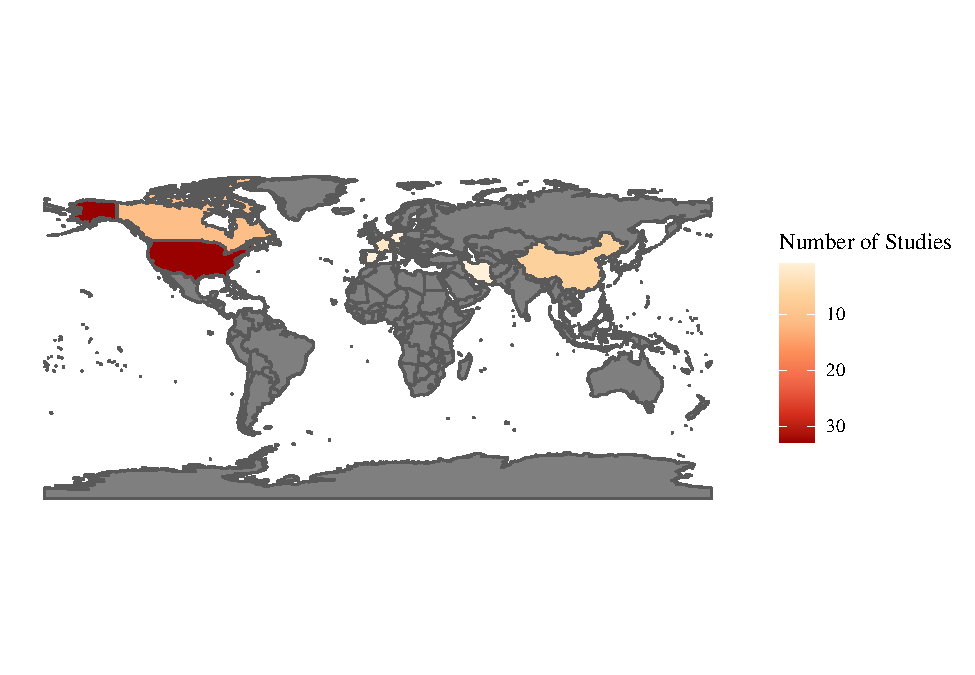
\includegraphics[width=1\linewidth]{man/figures/README-choropleth_study_count-1}

\hypertarget{age-distributions-of-lower-limits-and-upper-limits-of-age-range-density-and-histogram-plots}{%
\subsection{Age distributions of lower limits and upper limits of age
range (Density and Histogram
plots)}\label{age-distributions-of-lower-limits-and-upper-limits-of-age-range-density-and-histogram-plots}}

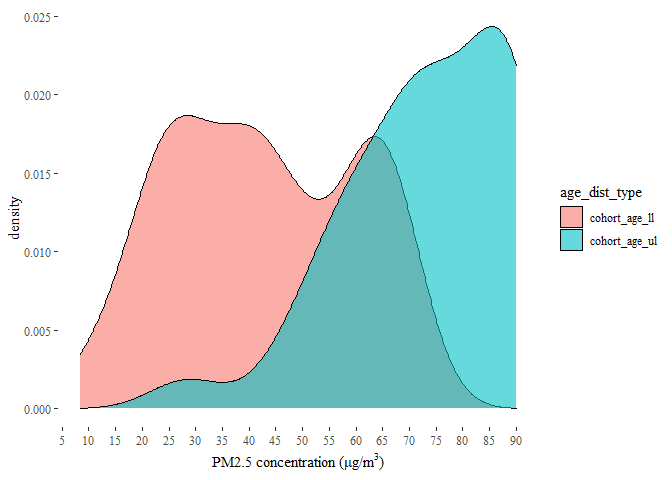
\includegraphics[width=1\linewidth]{man/figures/README-plot4_age_distribution_ll_ul-1}
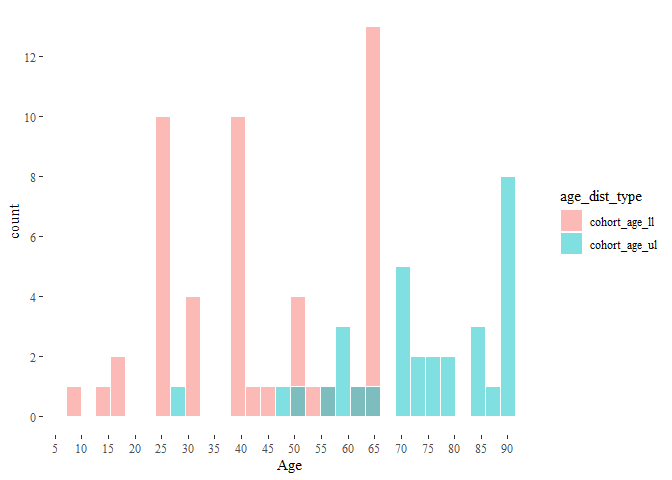
\includegraphics[width=1\linewidth]{man/figures/README-plot4_age_distribution_ll_ul-2}

\hypertarget{country-wise-distribution-of-cohort-sizes-density-and-histogram-plots}{%
\subsection{Country wise distribution of Cohort Sizes (Density and
Histogram
plots)}\label{country-wise-distribution-of-cohort-sizes-density-and-histogram-plots}}

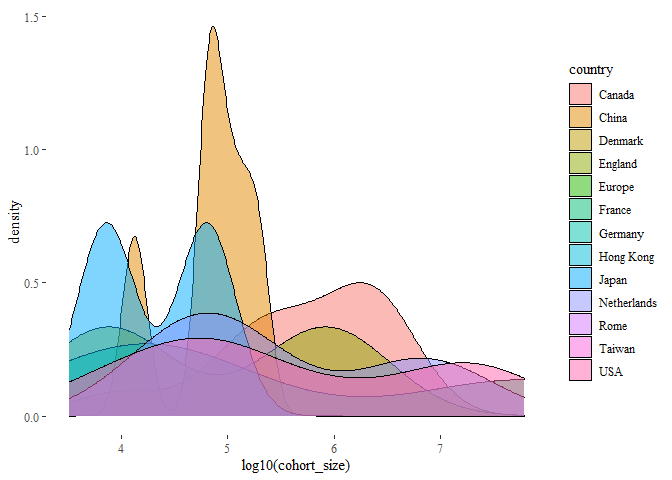
\includegraphics[width=1\linewidth]{man/figures/README-plot5_cohort_size_dist_country_wise-1}
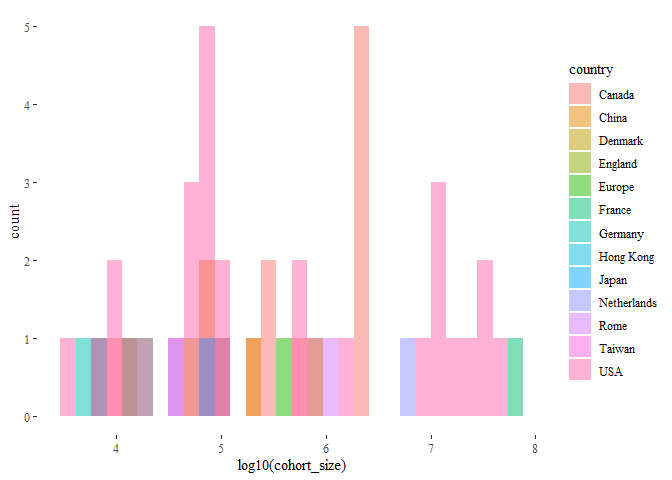
\includegraphics[width=1\linewidth]{man/figures/README-plot5_cohort_size_dist_country_wise-2}

\hypertarget{country-wise-distribution-of-study-duration-density-and-histogram-plots}{%
\subsection{Country wise Distribution of Study Duration (Density and
Histogram
Plots)}\label{country-wise-distribution-of-study-duration-density-and-histogram-plots}}

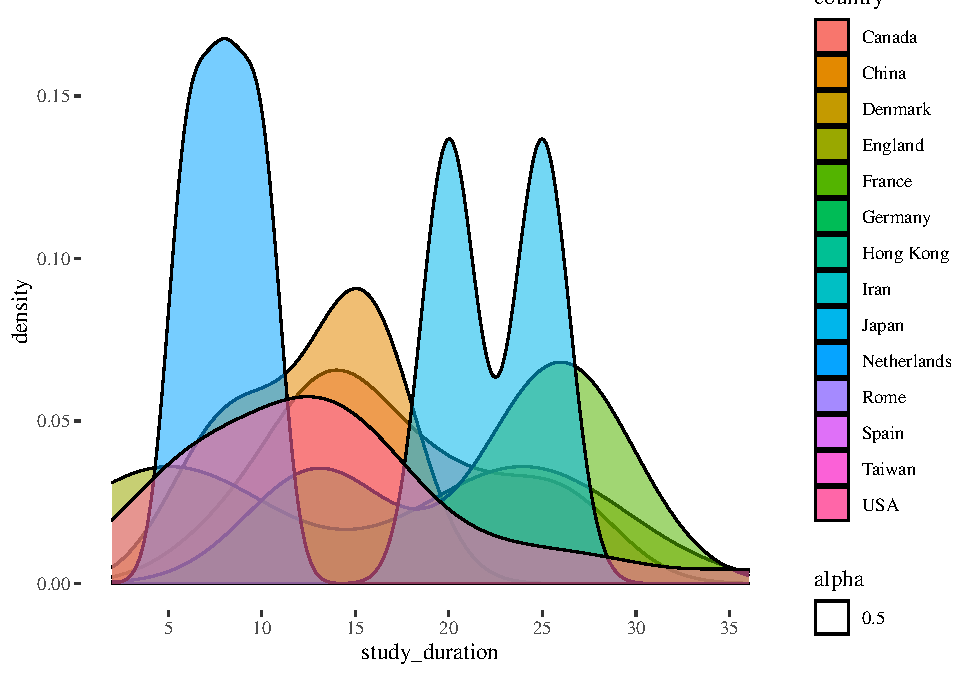
\includegraphics[width=1\linewidth]{man/figures/README-study_duration_dist_country_wise-1}
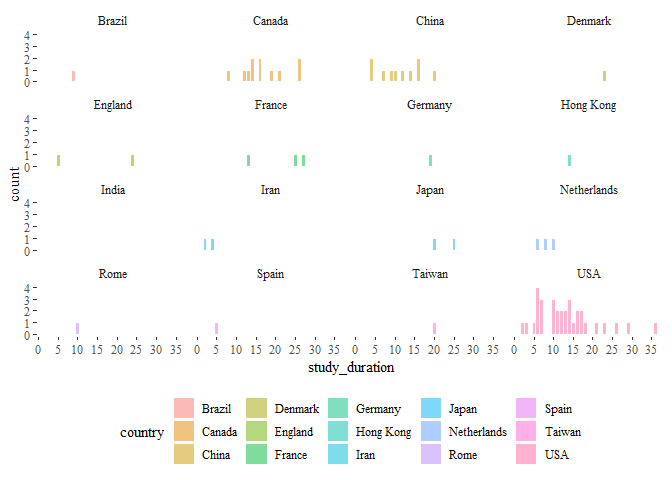
\includegraphics[width=1\linewidth]{man/figures/README-study_duration_dist_country_wise-2}

\hypertarget{aqli-data-top-10-most-polluted-countries-pm2.5-distributions-histograms-and-summary-table}{%
\subsection{AQLI data, top 10 most polluted countries: PM2.5
distributions Histograms and Summary
Table}\label{aqli-data-top-10-most-polluted-countries-pm2.5-distributions-histograms-and-summary-table}}

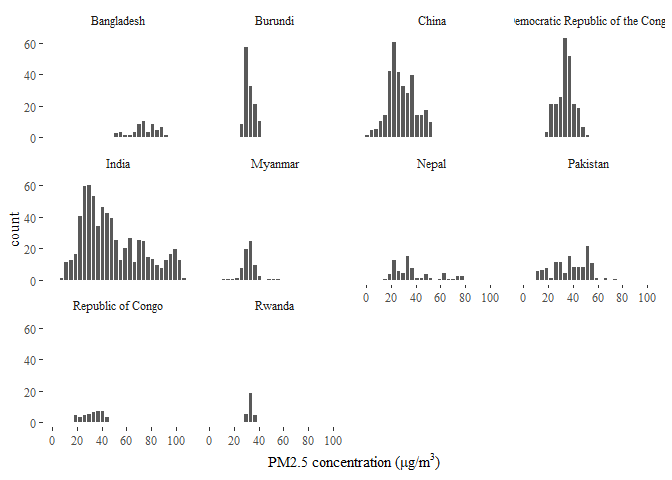
\includegraphics[width=1\linewidth]{man/figures/README-pm2.5_country_dist_aqli_plot-1}

\hypertarget{summary-table}{%
\subsubsection{Summary Table}\label{summary-table}}

\begin{longtable}[]{@{}lr@{}}
\toprule
Country & Average PM2.5 2020 (µg/m³) \\
\midrule
\endhead
Bangladesh & 75.75863 \\
India & 55.79855 \\
Nepal & 47.12727 \\
Pakistan & 44.17125 \\
Democratic Republic of the Congo & 34.19913 \\
Rwanda & 32.95480 \\
Myanmar & 32.43946 \\
Burundi & 31.76077 \\
China & 31.63255 \\
Republic of Congo & 31.62412 \\
\bottomrule
\end{longtable}

\end{document}
